%\documentclass[wsdraft]{ws-procs11x85}

\documentclass{ws-procs11x85}
\usepackage{ws-procs-thm}           % comment this line when `amsthm / theorem / ntheorem` package is used

\usepackage{lmodern}
\usepackage{amssymb,amsmath}
\usepackage{ifxetex,ifluatex}
\ifnum 0\ifxetex 1\fi\ifluatex 1\fi=0 % if pdftex
  \usepackage[T1]{fontenc}
  \usepackage[utf8]{inputenc}
  \usepackage{textcomp} % provides euro and other symbols
\else % if luatex or xelatex
  \usepackage{unicode-math}
  \defaultfontfeatures{Scale=MatchLowercase}
  \defaultfontfeatures[\rmfamily]{Ligatures=TeX,Scale=1}
\fi
% use upquote if available, for straight quotes in verbatim environments
  \usepackage[]{microtype}
  \UseMicrotypeSet[protrusion]{basicmath} % disable protrusion for tt fonts

\usepackage{xcolor}
\IfFileExists{bookmark.sty}{\usepackage{bookmark}}{\usepackage{hyperref}}
\hypersetup{
  pdftitle={Expanding polygenic risk scores to include automatic genotype encodings and gene-gene interactions},
  pdfauthor={Trang T. Le},
  pdfkeywords={markdown, publishing, manubot},
  pdfborder={0 0 0},
  breaklinks=true}
\urlstyle{same}  % don't use monospace font for urls
\usepackage{graphicx,grffile}

\begin{document}

\title{Expanding polygenic risk scores to include\\
automatic genotype encodings and gene-gene interactions}

\author{Trang T. Le$^\dag$, Hoyt Gong$^\dag$, Patryk Orzechowski, Elisabetta Manduchi}

\address{Department of Biostatistics, Epidemiology and Informatics,\\
University of Pennsylvania, Philadelphia, PA 19104}

\author{Jason H. Moore*}

\address{Department of Biostatistics, Epidemiology and Informatics,\\
Institute for Biomedical Informatics\\
University of Pennsylvania, Philadelphia, PA 19104\\
Email: jhmoore@upenn.edu}

\begin{abstract}
Polygenic Risk Scores (PRS) are aggregation of genetic risk factors of
specific diseases and have been successfully used to identify groups
of individuals who are more susceptible to those diseases. While several
studies have focused on identifying the correct genetic variants to
include in PRS, most existing statistical models focus on the marginal
effect of the variants on the phenotypic outcome but do not account for
the effect of gene-gene interactions. Here, we propose a novel
calculation of the risk score that expands beyond marginal effect of
individual variants on the outcome. The Multilocus Risk Score
(MRS) method effectively selects alternative genotype encodings and
captures epistatic gene-gene interactions by utilizing an efficient
implementation of the model-based Multifactor Dimensionality Reduction
technique. On a diverse collection of datasets, MRS outperforms the
standard PRS in the majority of the cases, especially when at least
two-way interactions between the variants are present. Our findings suggest
that models incorporating epistatic interactions are
necessary and will yield more accurate and effective risk profiling.
\end{abstract}

\keywords{GWAS; risk profiling; complex diseases; epistasis}

% required, do-not-remove
\copyrightinfo{\copyright\ 2016 The Authors. Open Access chapter published by World Scientific Publishing Company and distributed under the terms of the Creative Commons Attribution Non-Commercial (CC BY-NC) 4.0 License.}

\section{Introduction}\label{introduction}

As the field of traditional genomics rapidly expands its sequencing
technologies and translational abilities, novel applications of genomic
data are starting to arise in addressing disease burden. Complementing
the rapid growth in our understanding of human genetic variation was the
emergence of genome-wide association studies (GWAS) in the early 2000s
to identify gene variants associated with common human diseases.
Non-candidate-driven in design, these observational studies carry out
chip array genotyping across population subsamples to subsequently assay
for phenotype signal association via statistical approaches in silico.
Measuring averaged allelic effects across all genomics backgrounds and
environmental exposures, GWAS have primarily sought to discern genetic
association with phenotypes of interest by studying single nucleotide
polymorphisms (SNPs) and other DNA variants across the human genome
(Bush and Moore, \protect\hyperlink{ref-iFUfVw9V}{2012}; Hirschhorn and
Daly, \protect\hyperlink{ref-5cdeEdUS}{2005}; Wang \emph{et al.},
\protect\hyperlink{ref-12kQ0EOWQ}{2005}).

In tandem with the movement towards precision medicine, the post-GWAS
era strives to bring relevant population-derived gene variants into
individual level metrics actionable in health delivery settings. While
GWAS indeed capture gene variants associated with a phenotype of
interest on a population level, translating such results to personalized
individual metrics of risk requires aggregating contributions of many
gene variants in the form of polygenic risk scores (PRS). PRS provide an
ability to explain inherited risk for disease in an individual by
representing a weighted sum aggregate of risk alleles based on measured
loci effect contributions derived from GWAS (Chatterjee \emph{et al.},
\protect\hyperlink{ref-auyRflEe}{2016}; Torkamani \emph{et al.},
\protect\hyperlink{ref-1GK3F1BxE}{2018}). In quantifying the effect of
particular combinations of genetic SNP variants towards risk prediction,
PRS offers a probabilisitic susceptibility value of an individual to
disease. Such genetic risk estimation scores are central to clinical
decision-making, serving to reinforce individual health management in
heritable disease detection and early prevention of various adult-onset
conditions. The utility of PRS scores have been demonstrated in previous
studies towards disease risk stratification across leading heritable
causes of death in the developed world
(\protect\hyperlink{ref-mwTa2RUK}{2009}; Khera \emph{et al.},
\protect\hyperlink{ref-oBD9eYkN}{2019},
\protect\hyperlink{ref-Gh0gKn77}{2018}; Maas \emph{et al.},
\protect\hyperlink{ref-Z12fynub}{2016}; Seibert \emph{et al.},
\protect\hyperlink{ref-gkABDVTx}{2018}).

Because common PRS method assumes a simplified genetic architecture
consisting of independent weights, understanding interactive
relationships among genes and SNPs that associate with disease outcome
remain a challenge. Existing standard multivariate categorical data
analysis approaches fall short in handling such enormous possible
genetic interaction combinations with both linear and nonlinear effects.
In this context, more robust and efficient methods towards a polygeneic
risk calculation are necessary in capturing the overlap between
context-dependent effects of both rare and common alleles on human
genetic disorder. Herein, we use the terminology gene-gene (GxG)
interactions to indicate any genetic interaction including ones among
SNPs that may fall outside of coding regions.

With respect to better understanding the epistasis across an
individual's genome, various statistical models have been designed with
the intent of capturing high dimensional GxG interactions. The
Multifactor Dimensionality Reduction (MDR) method is one such
nonparametric framework that addresses these challenges and has been
extensively applied to detect nonlinear complex GxG interactions
associated with individual disease (Ritchie \emph{et al.},
\protect\hyperlink{ref-E26QhGxD}{2001}; Moore and Andrews,
\protect\hyperlink{ref-1BqLrlGsj}{2014}). By isolating a specific pool
of genetic factors from all polymorphism and cross-valiating prediction
scores averaged across identified high risk multi-locus genotypes, the
original MDR approach is able to categorize multilocus genotypes into
two groups of risk based on a threshold value. While created with the
primary intention towards GxG interaction detection by reducing
dimensionality interactively in inferring genotype encodings, the MDR
model has additionally demonstrated applicability as a risk score
calculation model in constructing PRS scores (Dai \emph{et al.},
\protect\hyperlink{ref-93PfLXPZ}{2013}).

Modifications built on top of the MDR framework have been proposed in
order to better capture multiple significant epistasis models and
potential missed interactions owning to limitations of the original
model in the higher dimensions. Model-Based Multifactor Dimensionality
Reduction (MB-MDR) was formulated as a flexible GxG detection framework
for both dichotomous and continuous traits (Mahachie John \emph{et al.},
\protect\hyperlink{ref-kN4MaLuT}{2011}; Cattaert \emph{et al.},
\protect\hyperlink{ref-16AnEAMje}{2010}). Rather than a direct
comparison against a threshold level in the original MDR method, MB-MDR
merges multilocus genotypes exhibiting significant High or Low risk
levels through association testing and adds an additional `No evidence
of risk' categorization. In comparison to the standard MDR framework
which reveals at most one optimal epistasis model, the MB-MDR method
flexibly weighs multiple models by producing a model list ranked with
respect to their statistical parameters.

In the present work, we aim to reformulate the PRS leveraging the MB-MDR
approach to better capture alternative encodings and epistatic
interactions of individual disease risk in a novel Multilocus Risk Score
(MRS). Through the following sections, we briefly review the features of
the MDR and MB-MDR software, describe how our new MRS method evaluates
polygenic risk, and compare MRS profiling performance to the standard
PRS method on evidence-based simulated dataset collections. In observing
prediction accuracy results, we demonstrate the improved performance of
our multi-model weighted epistasis framework with inferred genotype
encodings over existing PRS methods, showing great potential for more
accurate identification of high risk individuals for a specific complex
disease.

\section{Methods}
\subsection{Multifactor Dimensionality Reduction (MDR) and
model-based MDR
(MB-MDR)}\label{multifactor-dimensionality-reduction-mdr-and-model-based-mdr-mb-mdr}
MDR is a nonparametric method that detects multiple genetic loci
associated with a clinical outcome by reducing the dimension of a
genotype dataset through pooling multilocus genotypes into high-risk and
low-risk groups (Ritchie \emph{et al.},
\protect\hyperlink{ref-E26QhGxD}{2001}). Extended from the original MDR
algorithm, MB-MDR was first introduced in 2009, and its current
implementation efficiently and effectively detects multiple sets of
significant gene-gene interactions in relation to a trait of interest
while efficiently controlling type I error rates.

In addition to the test statistic and P values associated with each
genotype combination, another important output of MB-MDR is the HLO
matrices. Briefly, in the case of a binary trait, for each genotype
combination, an HLO matrix is a 3 x 3 matrix with each cell containing H
(high), L (low) or O (no evidence), indicating risk of an individual
whose genotype pairs fall into that cell (Lishout \emph{et al.},
\protect\hyperlink{ref-S6nj6BFK}{2013}). For an example binary outcome
problem, a genotype combination \(SNP_1\) and \(SNP_2\) will have an HLO
matrix that looks like \[ \begin{array}{l|ccc}
& \, SNP_1 = 0 \quad& SNP_1 = 1 \quad& SNP_1 = 2  \quad \\
\hline
SNP_2 = 0 \,\,& O        & O        & O \\
SNP_2 = 1 \,\,& O        & H        & L \\
SNP_2 = 2 \,\,& O        & L        & H
\end{array}
\] We discuss in the following subsection how these values were utilized
in the formulation of the Multilocus Risk Score (MRS).


\subsection{From Polygenic Risk Scores (PRS) to Multilocus Risk
Scores
(MRS)}\label{from-polygenic-risk-scores-prs-to-multilocus-risk-scores-mrs}

In this subsection, we quickly review the standard PRS formula then
present our modification to this popular risk score calculation. For
both methods, we consider a dataset of \(n\) individuals with genomes of
\(m\) possible SNPs.

In PRS, for each SNP \(j\) of an individual \(i\), the PRS score is
calculated via a summation across \(k\) selected SNPs as
\[PRS(i)=\sum_{j=1}^{k} \beta_j \times SNP_{ij}\] where \(\beta_j\) is
the weighted risk contribution of the \(j^\textrm{th}\) SNP derived from
the association test parameters and \(SNP_{ij}\) represents the number
of minor alleles (0, 1, or 2) at the \(j^\textrm{th}\) locus of
individual \(i\). Various approaches towards predicting risk of the same
disease exist across PRS studies based on the above equation; models may
vary according to the specific statistical model used to produce the
weights \(\beta_j\) for individual genetic variations, the number of
genetic variants considered \(k\), and the ability of the PRS to
generalize to the entire population (Sugrue and Desikan,
\protect\hyperlink{ref-1Dlv3tAGh}{2019}).

In the MRS framework, we let \(k_d\) denote the number of significant
combinations for a specific model dimension \(d\) (e.g.~\(d = 2\)
results in pairs of SNPs). In this study, no significance threshold is
imposed at the SNP combination level and, thus, \(k_d\) reaches its
maximum value of \(C^d_m\) (\(m\) choose \(d\)). For each subject \(i\)
(\(i = 1,2, \dotsm, n\)), the \(d\)-way multilocus risk score is
calculated as
\[MRS_d(i) = \sum_{j = 1}^{k_d} \gamma_j \times \textrm{HLO}_j(X_{ij})\]
where \(\gamma_j\) is the test statistic of the \(j^\textrm{th}\)
genotype combination output from MB-MDR, \(X_{ij}\) is the
\(j^\textrm{th}\) genotype combinations of subject \(i\) and
\(\textrm{HLO}_j\) represents the \(j^\textrm{th}\) recoded HLO matrix
(1 = High, -1 = Low, 0 = No evidence). As an example, consider a pair
\(X_{*j} = (SNP_{j_1}, SNP_{j_2})\) with \(\gamma_j=8.3\) and
corresponding HLO matrix of all O's except an L in the first cell. Then,
all subjects' current risks would remain the same except the ones with
\(SNP_{j_1} = SNP_{j_2} = 0\) where their risks are subtracted by 8.3.

In this study, we consider 1-way and 2-way interactions. We denote by
MRS the combined risk score MRS1 + MRS2. The significance level of each
combination of SNPs on a given dataset is obtained by applying on that
dataset the MB-MDR software (Lishout \emph{et al.},
\protect\hyperlink{ref-S6nj6BFK}{2013}; Cattaert \emph{et al.},
\protect\hyperlink{ref-16AnEAMje}{2010}) v.4.4.1. We will compare the
performance of the standard PRS method to the combined risk MRS and also
its components, MRS1 and MRS2, separately.

\subsection{Mutual information and information
gain}\label{mutual-information-and-information-gain}

For a given simulated data set, we apply entropy-based methods to
measure how much information about the phenotype is due to either
marginal effects or the synergistic effects of the variants after
subtracting the marginal effects. A dataset's amount of main effect
\(ME\) can be measured as the total of mutual information between each
genotype \(SNP_j\) and the phenotypic class \(Y\) based on Shannon's
entropy \(H\) (Shannon, \protect\hyperlink{ref-yzGboP1g}{1948}):
\[ME = \sum_{j}^k I(SNP_j; Y) = \sum_{j}^k H(Y) - H(Y|SNP_j).\]

We measure the 2-way interaction information (i.e.~degree of synergistic
effects of genotypes on the phenotype) of each dataset by summing the
pairwise information gain between all pairs of genetic attributes.
Specifically, if we let \(X_j\) denote the \(j^\textrm{th}\) genotype
combination \((SNP_{j_1}, SNP_{j_2})\), the total 2-way interaction gain
(i.e.~synergistic effects \(SE\)) is calculated as
\[SE = \sum_{j}^kIG(X_j; Y) = \sum_{j}^k \left(I(SNP_{j_1}, SNP_{j_2}; Y) - I(SNP_{j_1}; Y) - I(SNP_{j_2}; Y)\right),\]
where \(IG\) measures how much of the phenotypic class \(Y\) can be
explained by the 2-way epistatic interaction within the genotype
combination \(X_j\). We refer the reader to Ref. (Moore and Hu,
\protect\hyperlink{ref-1FFMLUZxb}{2014}) for more details on the
calculation of the entropy-based terms.

To prevent potential bias, we compute these values from the training set.
However, because the training and holdout sets were randomly split, the amount of main or interaction effect in both datasets are expected to be similar.

\subsection{Simulated data}\label{simulated-data}

The primary objective of this data simulation process was to provide a
comprehensive set of reproducible and diverse datasets for the current
study. Each dataset was generated in the following manner. For an
individual, each genotype was randomly assigned with 1/2 probability of
being heterozygous (\emph{Aa}, coded as \texttt{1}), 1/4 probability of
being homozygous major (\emph{AA}, coded as \texttt{0}) and 1/4
probability of being homozygous minor (\emph{aa}, coded as \texttt{2}).
The binary endpoint for the data was determined using a recently
proposed evolutionary-based method for dataset generation called
Heuristic Identification of Biological Architectures for simulating
Complex Hierarchical Interactions (HIBACHI) (Moore \emph{et al.},
\protect\hyperlink{ref-pDXdtMFa}{2017}). Details on data simulation are
provided in the README of the study's analysis repository
\url{https://github.com/lelaboratoire/rethink-prs/}.

The final collection has 450 datasets containing 1000 samples and 10
SNPs with various amount of epistatic effect on the binary phenotypic
outcome. For each simulated dataset, after randomly splitting the entire
data in two smaller sets (80\% training and 20\% holdout), we built the
MRS model on training data to obtain the \(\gamma\) coefficients and the
HLO matrices, and then we calculated risk score for each sample in the
holdout set. We assess the performance of the MRS by comparing the area
under the Receiving Operator Characteristic curve (auROC) with that of
the standard PRS method on the holdout set.

\subsection{Manuscript drafting}\label{manuscript-drafting}


This manuscript is collaboratively written using Manubot, a software for
writing scholarly documents via GitHub (Himmelstein \emph{et al.},
\protect\hyperlink{ref-YuJbg3zO}{2019}). With continuous integration,
Manubot automatically updates the manuscript when its authors approve
the changes. As a result, the latest version of this manuscript is
always available for review at
\url{https://lelaboratoire.github.io/rethink-prs-ms/}.


\subsection{Availability}\label{availability}

Detailed simulation and analysis code needed to reproduce the results in
this study is available at
\url{https://github.com/lelaboratoire/rethink-prs/}.


\section{Results}\label{results}

\subsection{MRS outperforms standard PRS in the majority of simulated
datasets}\label{mrs-outperforms-standard-prs-in-the-majority-of-simulated-datasets}

In 335 out of 450 simulated datasets, MRS produces higher auROC compared
to PRS (green lines, Fig. \ref{fig:auroc_mrs_prs}). In 363 datasets
where the standard PRS method performs poorly (auROC \textless{} 60\%),
MRS performs particularly well (auROC \textgreater{} 90\%) in 102
datasets. This auROC increase of approximately 50\% can be seen at the second peak in the density of the difference between the auROCs from the two methods (Fig. \ref{fig:auroc_mrs_prs} right).
When MRS yields smaller auROC, the difference is small (3.3\%
± 2.8\%, purple lines/areas). Across all 450 datasets, the improvement of
MRS over PRS is significant (P \textless{} \(10^{-15}\)) according to a
Wilcoxon signed rank test. To assess whether this improvement in
performance correlates with the amount of interaction effect contained
in each dataset, in the following section, we untangled the two
components of MRS and test for the correlation between the difference in
auROC and two entropy-based measures for main and interaction effect of
each dataset.

\begin{figure}
\centering
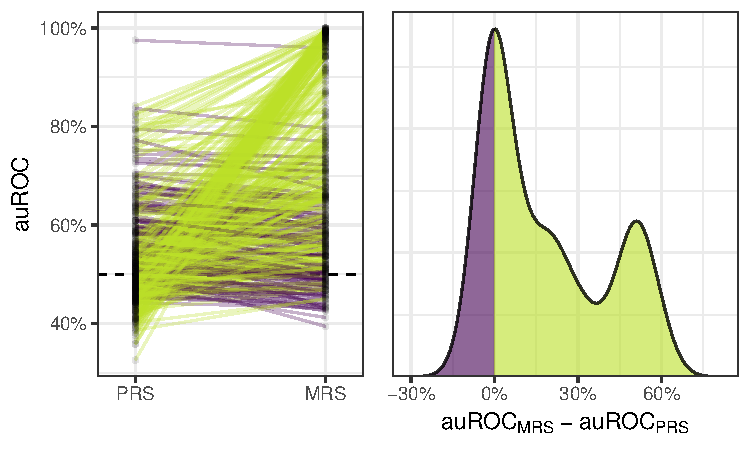
\includegraphics[width=0.8\textwidth]{../content/images/1_ori_vs_MRS_auROC_.pdf}
\caption{MRS produces improved auROC in the majority (335 green lines)
of the 450 simulated datasets (each line represents a dataset). In many
datasets, the standard PRS method performs poorly (auROC \textless{}
60\%) while the new method yields auROC over 90\%. This improvement in
performance can be seen at the second peak (\textasciitilde{}50\% auROC
increase) in the density of the difference between the auROCs from the
two methods (right).}
\label{fig:auroc_mrs_prs}
\end{figure}

\hypertarget{assess-improvement-in-performance}{%
\subsection{Assess MRS's improvement in
performance}\label{assess-improvement-in-performance}}

We recall that MRS is combined from the 1-way and 2-way interaction risk scores: MRS = MRS1 + MRS2.
Individually, MRS1 and MRS2 both significantly outperformed the standard
PRS method (both P values \textless{} \(10^{-15}\)) according to a
Wilcoxon signed rank test. As the amount of main effect increases (Fig.
\ref{fig:improvements} left column), MRS1 increasingly performs better
than PRS, which is likely because encodings are inferred (top left).
Meanwhile, MRS2's accuracy remain mostly similar to that of PRS (middle
left). On the other hand, when the amount of interaction effect
increases (Fig. \ref{fig:improvements} right column), MRS1 performs
mostly on par to PRS while MRS2 increasingly performs better than PRS.
Combining the gain from both MRS1 and MRS2, MRS's performance
progressively increases compared to the standard PRS.

\begin{figure}
\centering
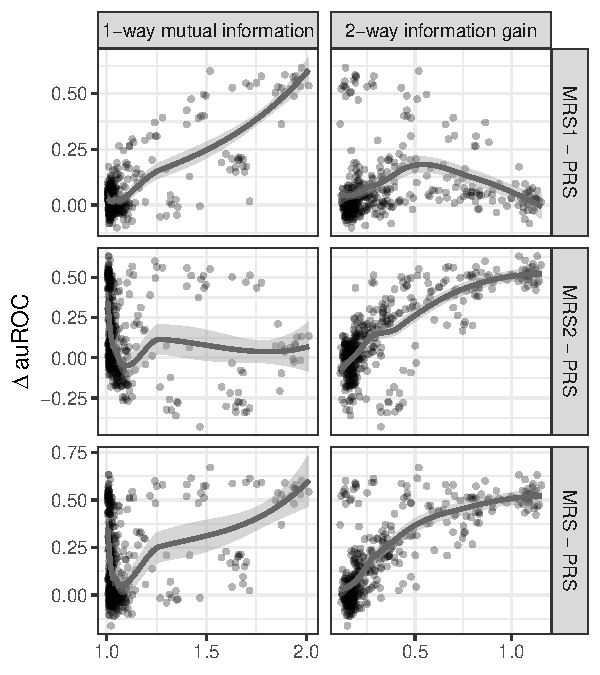
\includegraphics[width=0.7\textwidth]{../content/images/improvements_train_ms.pdf}
\caption{Combining 1-way (MRS1) and 2-way (MRS2) risk scores, MRS shows
increasing outperformance to standard PRS as datasets contain more main
and interaction effect.\label{fig:improvements}}
\end{figure}

\hypertarget{discussion}{%
\section{Discussion}\label{discussion}}

We introduce the Multilocus Risk Score (MRS) method to improve the
performance of the standard PRS in disease risk stratification of
patient populations. While PRS holds much promise for development of new
precision medicine approaches by identifying high risk individuals, one of its current
limitations is the model simplicity (Torkamani \emph{et al.},
\protect\hyperlink{ref-1GK3F1BxE}{2018}). As a first step towards
addressing this issue and increasing comprehensiveness of risk profiling
models, in this study, we developed a new applied MRS method from the
MB-MDR framework that enables automatic genotype encodings and takes
into account multiple models for detecting GxG interactions. Utilizing
the efficient implementation of MB-MDR, MRS automatically infers the
genotype encodings and simultaneously computes the risk of variant
combinations. Through comparing method performance on a diverse
collection of simulated data, we demonstrate the robust risk
profiling ability of MRS and suggest the importance of flexible, precise
methods in better capturing epistasis behind individual patient risk.

We showed that the MRS method outperformed standard PRS in many of the
simulated datasets, highlighting the importance of genotype encodings
and consideration of epistasis. We further examined the association
between this improvement and the amount of two-way epistatic effect
induced in the binary phenotypic outcome. Appropriate phenotype
encodings are important for improving the accuracy when there is a large
amount of main effect of the variants on the phenotypic outcome.
Meanwhile, inclusion of epistatic terms significantly increases the
accuracy from PRS, especially when two-way interactions are present in
the data. Although we only considered up to two-way GxG interactions, it
is straightforward to incorporate higher order interactions
(e.g.~three-way, four-way) into MRS. However, preliminary analyses on
the simulated datasets for such higher order interactions did not show
significant improvement from the current MRS (results not shown). We
also recommend estimating the computational expense prior to
implementing high order interactions, especially for larger datasets
encountered in practice.

We acknowledge three main limitations of the current study. First, MRS has not
been applied to real-world data. Although we compensated the lack of
real data with a diverse set of simulated datasets, a future study
analyzing real-world data will prove beneficial to quantify the new MRS
model's utility in practice. Second, accounting for epistasis, in
principle, is more computationally expensive compared to
investigating solely main effect. Therefore, even with fast and
efficient software, pre-selecting the variants (e.g.~based on specific
pathways or prior knowledge) will prove beneficial for accurate MRS
computing when analyzing datasets containing a larger number of
variants. Nevertheless, we hope the promising preliminary results from
this study will open the door to future approaches that encompass both
main and interaction effects while improving scalability.

Finally, we caution that a risk score model should be evaluated based on
not only sensitivity and specificity but also with respect to potential
clinical efficacy, and any genetic risk should be interpreted in
aggregate with other risk factors. Future works focusing on
gene-environment interactions with time-dependent risk factors will be
crucial in order to communicate risk properly for preventive
interventions.

In conclusion, MRS enhances the predictive capacity of current risk
profiling model for complex diseases with polygenic architectures. While
there is much work left to do in improving the clinical
utility of general risk profiling framework, we highlight that more
comprehensive models that infer proper genotype encodings and account
for epistatic effects greatly improve the prediction accuracy and
affords new opportunities for more effective clinical prevention.

\hypertarget{acknowledgement}{%
\section{Acknowledgements}\label{acknowledgement}}

We thank Dr.~Kristel Van Steen and Aldo Camargo for their helpful
responses to our inquires about the MB-MDR software.

\hypertarget{funding}{%
\section{Funding}\label{funding}}

This work was supported by the National Institutes of Health 
grant numbers LM010098, LM012601 and AI116794.

\hypertarget{references}{%
\section*{References}\label{references}}

\hypertarget{refs}{}
\leavevmode\hypertarget{ref-iFUfVw9V}{}%
Bush,W.S. and Moore,J.H. (2012) Chapter 11: Genome-Wide Association
Studies. \emph{PLoS Comput Biol}, \textbf{8}, e1002822.

\leavevmode\hypertarget{ref-16AnEAMje}{}%
Cattaert,T. \emph{et al.} (2010) Model-Based Multifactor Dimensionality
Reduction for detecting epistasis in case-control data in the presence
of noise. \emph{Annals of Human Genetics}, \textbf{75}, 78--89.

\leavevmode\hypertarget{ref-auyRflEe}{}%
Chatterjee,N. \emph{et al.} (2016) Developing and evaluating polygenic
risk prediction models for stratified disease prevention. \emph{Nat Rev
Genet}, \textbf{17}, 392--406.

\leavevmode\hypertarget{ref-93PfLXPZ}{}%
Dai,H. \emph{et al.} (2013) Risk score modeling of multiple gene to gene
interactions using aggregated-multifactor dimensionality reduction.
\emph{BioData Mining}, \textbf{6}.

\leavevmode\hypertarget{ref-YuJbg3zO}{}%
Himmelstein,D.S. \emph{et al.} (2019) Open collaborative writing with
Manubot. \emph{PLoS Comput Biol}, \textbf{15}, e1007128.

\leavevmode\hypertarget{ref-5cdeEdUS}{}%
Hirschhorn,J.N. and Daly,M.J. (2005) Genome-wide association studies for
common diseases and complex traits. \emph{Nat Rev Genet}, \textbf{6},
95--108.

\leavevmode\hypertarget{ref-Gh0gKn77}{}%
Khera,A.V. \emph{et al.} (2018) Genome-wide polygenic scores for common
diseases identify individuals with risk equivalent to monogenic
mutations. \emph{Nat Genet}, \textbf{50}, 1219--1224.

\leavevmode\hypertarget{ref-oBD9eYkN}{}%
Khera,A.V. \emph{et al.} (2019) Polygenic Prediction of Weight and
Obesity Trajectories from Birth to Adulthood. \emph{Cell}, \textbf{177},
587--596.e9.

\leavevmode\hypertarget{ref-S6nj6BFK}{}%
Lishout,F.V. \emph{et al.} (2013) An efficient algorithm to perform
multiple testing in epistasis screening. \emph{BMC Bioinformatics},
\textbf{14}.

\leavevmode\hypertarget{ref-Z12fynub}{}%
Maas,P. \emph{et al.} (2016) Breast Cancer Risk From Modifiable and
Nonmodifiable Risk Factors Among White Women in the United States.
\emph{JAMA Oncol}, \textbf{2}, 1295.

\leavevmode\hypertarget{ref-kN4MaLuT}{}%
Mahachie John,J.M. \emph{et al.} (2011) Model-Based Multifactor
Dimensionality Reduction to detect epistasis for quantitative traits in
the presence of error-free and noisy data. \emph{Eur J Hum Genet},
\textbf{19}, 696--703.

\leavevmode\hypertarget{ref-1BqLrlGsj}{}%
Moore,J.H. and Andrews,P.C. (2014) Epistasis Analysis Using Multifactor
Dimensionality Reduction. In, \emph{Methods in Molecular Biology}.
Springer New York, pp. 301--314.

\leavevmode\hypertarget{ref-1FFMLUZxb}{}%
Moore,J.H. and Hu,T. (2014) Epistasis Analysis Using Information Theory.
In, \emph{Methods in Molecular Biology}. Springer New York, pp.
257--268.

\leavevmode\hypertarget{ref-pDXdtMFa}{}%
Moore,J.H. \emph{et al.} (2017) A heuristic method for simulating
open-data of arbitrary complexity that can be used to compare and
evaluate machine learning methods. In, \emph{Biocomputing 2018}. WORLD
SCIENTIFIC.

\leavevmode\hypertarget{ref-E26QhGxD}{}%
Ritchie,M.D. \emph{et al.} (2001) Multifactor-Dimensionality Reduction
Reveals High-Order Interactions among Estrogen-Metabolism Genes in
Sporadic Breast Cancer. \emph{The American Journal of Human Genetics},
\textbf{69}, 138--147.

\leavevmode\hypertarget{ref-gkABDVTx}{}%
Seibert,T.M. \emph{et al.} (2018) Polygenic hazard score to guide
screening for aggressive prostate cancer: development and validation in
large scale cohorts. \emph{BMJ}, j5757.

\leavevmode\hypertarget{ref-yzGboP1g}{}%
Shannon,C.E. (1948) A Mathematical Theory of Communication. \emph{Bell
System Technical Journal}, \textbf{27}, 379--423.

\leavevmode\hypertarget{ref-1Dlv3tAGh}{}%
Sugrue,L.P. and Desikan,R.S. (2019) What Are Polygenic Scores and Why
Are They Important? \emph{JAMA}, \textbf{321}, 1820.

\leavevmode\hypertarget{ref-1GK3F1BxE}{}%
Torkamani,A. \emph{et al.} (2018) The personal and clinical utility of
polygenic risk scores. \emph{Nat Rev Genet}, \textbf{19}, 581--590.

\leavevmode\hypertarget{ref-12kQ0EOWQ}{}%
Wang,W.Y.S. \emph{et al.} (2005) Genome-wide association studies:
theoretical and practical concerns. \emph{Nat Rev Genet}, \textbf{6},
109--118.

\leavevmode\hypertarget{ref-mwTa2RUK}{}%
Purcell,S.M. \emph{et al.} (2009) Common polygenic variation contributes to risk of schizophrenia
and bipolar disorder. \emph{Nature}, \textbf{460}, 748--752.

\end{document} 

%%% \renewcommand\bibname{References\\ {\normalfont\it References can be typed in your preferred bibliography style.}}